\chapter{Input Data}
\section{Problem 1: Simple network}
\section{Problem 2: Backpropagation}
\section{Problem 3: Artificial neural network}
\section{Problem 4: Gradient Descent}

The input data set consists of 1000 generated points with a $X$ value between $-5$ and $5$.
The $Y$ value is calculated with the formula $ y = mx + c $ where $m$ and $c$ are assumed by us.
Applying a random noise leads to the dataset which is shown in Figure \ref{problem4_imput_data}

\begin{figure}[h]
	\centering
	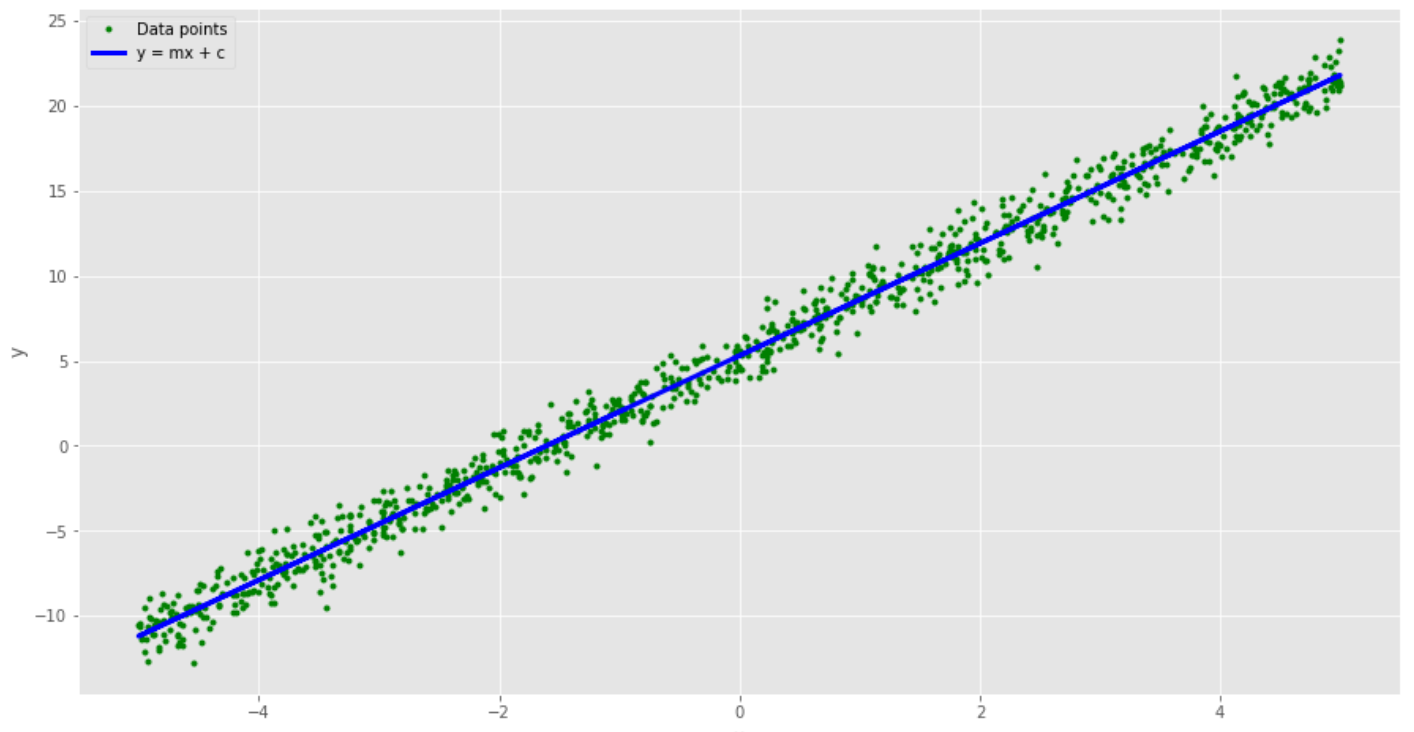
\includegraphics[height=8cm]{img/problem4_imput_data.png}
	\caption{Generated input data of problem 4}
    \label{problem4_imput_data}
\end{figure}

Further a jupyter notebook is provided which generate these data and provides a script which only need to be completed with the calculation of the gradient and updating and weight update for $m$ and $c$.

